\chapter{Bidirectional Long Short Term Memory Network Models}
In this chapter, we first describe Bidirectional Long Short Term Memory network (BiLSTM) and Character Embeddings. Then, we show the performance and decoding speed of BiLSTM models with different configurations on POS and NER.

\section{Model Description}
\subsection{Bidirectional Bidirectional Long Short Term Memory}

One major disadvantage of feedforward neural networks is that they only consider the context of the focused word instead of the whole sentence. Recurrent neural networks (RNNs) (\citeauthor{mikolov2010recurrent}, \citeyear{mikolov2010recurrent}) can keep the future and the past data persistent by using memory cells with loops in them. However, RNNs are biased towards the most recent data in practice. Long Short Term Memory Networks (LSTMs), special RNNs with Long Short Term memory cells  (\citeauthor{graves2005framewise}, \citeyear{graves2005framewise}), are designed to combat the bias problem. LSTMs learn long dependencies in a sequence with the help of Gates (\citeauthor{graves2005framewise}, \citeyear{graves2005framewise}). Gates control how much of the input information to pass to the next LSTM cell, and how much of the previous information to forget.

Given a sentence with $n$ words each of which is represented as a dense vector $x_i$, a LSTM makes use of $x_{1:n}$ to compute a forward representation $\overrightarrow {h_{i}}$ for the $i$th word. In general, computing a backward representation $\overleftarrow {h_{i}}$ would be useful for sequence tagging. Bidirectional LSTM (BiLSTM) is an extension to LSTM which takes into account both the past elements and the future elements in a sequence. A BiLSTM generates both $\overrightarrow {h_{i}}$ and $\overleftarrow {h_{i}}$ for the $i$th word in a sequence. The hidden embedding $h_{i}$ is the concatenation of $\overrightarrow {h_{i}}$ and $\overleftarrow {h_{i}}$. BiLSTM mapping is defined as $BiLSTM_{\theta}$:
$h_{i} = BiLSTM_{\theta}\left(x_{1:n}, i\right)$ where $\theta$ represents trainable parameters in BiLSTM.

 We can combine BiLSTM with CRF to make use of sentence level tag information. As in the Feedforward-CRF model, we introduce a transition matrix $T$ to keep the transition score from $y_{i}$ to $y_{i+1}$. Given an output sequence $Y$, the score of the output sequence is given by:

\begin{equation}
S\left( X|Y\right)=\sum _{i}^{n}T_{i,i+1}+\sum _{i}^{n}P_{i}
\end{equation}

We can use the dynamic programming algorithm to compute the transition matrix and find the optimal output tag sequence. Figure \ref{fig:bilstmcrf} illustrates the BiLSTM model with CRF on an NER example.

\begin{figure}
  \centering
  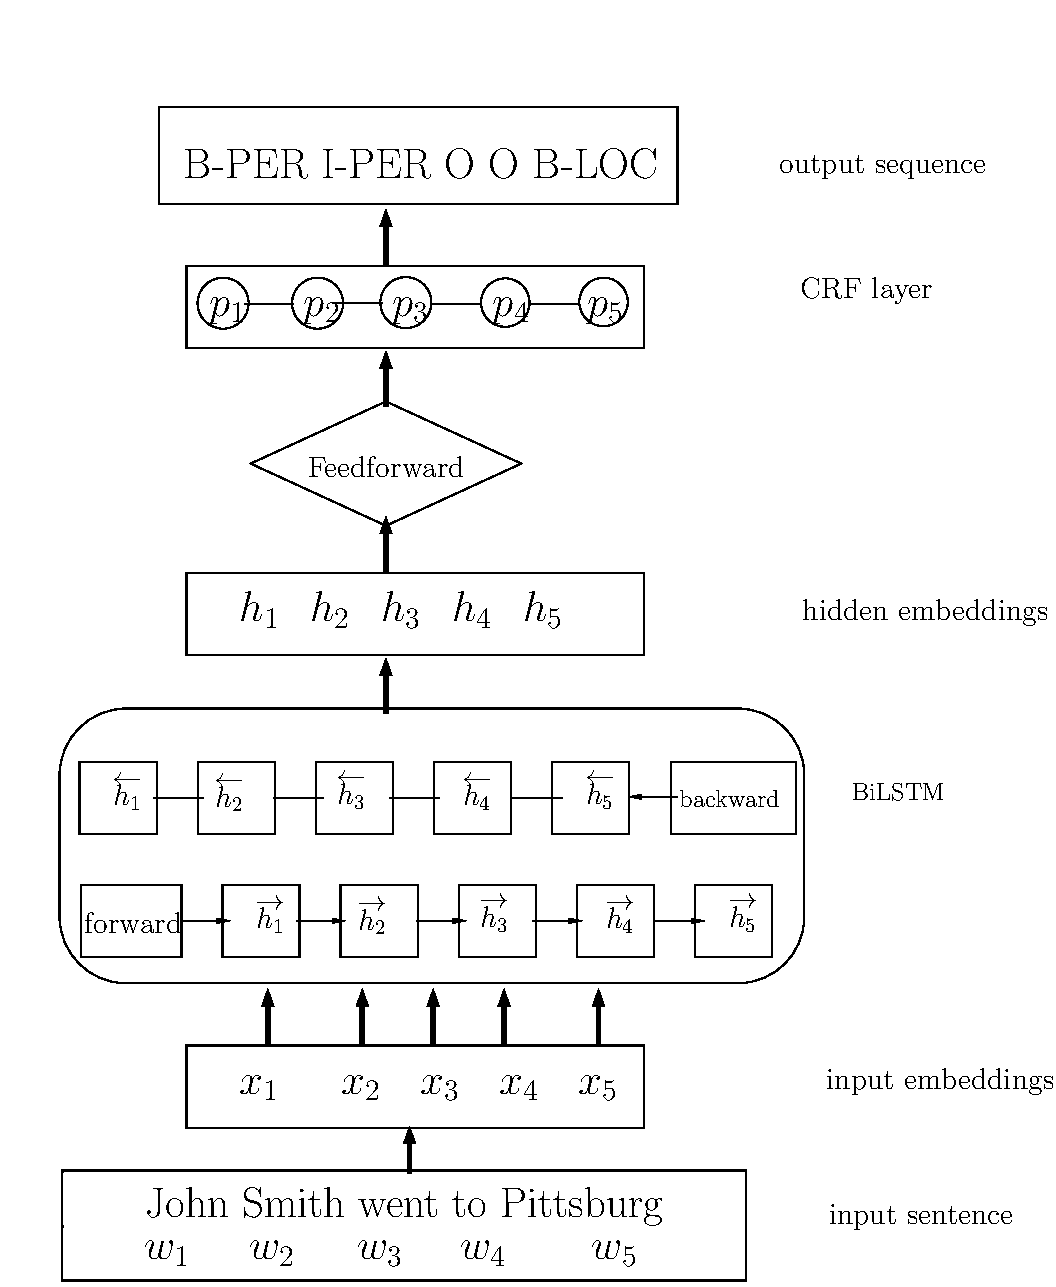
\includegraphics[scale=0.6]{bilstmcrf.pdf}
 \caption{The architecture of an NER tagging system using BiLSTM with CRF}
  \label{fig:bilstmcrf}
\end{figure}

\subsection{Character Embeddings}

Instead of using hand-engineered features listed in Chapter 2 (like prefixes and the suffixes of a word), we can use a BiLSTM network to construct word representations from characters in it (\citeauthor{lample2016neural}, \citeyear{lample2016neural}). This architecture is denoted as Character Embeddings. It has been shown that learning character embeddings has been found useful for capturing morphological evidence (\citeauthor{ling2015finding}, \citeyear{ling2015finding}). Figure \ref{fig:charlstm} describes the architecture using character embeddings and BiLSTM to generate word embedding for word "Smith". The input to the BiLSTM is the letter sequence of a word. We define a character dictionary which maps each character to a $d$-dimensional vector representation. The English character dictionary contains uppercase and lowercase letters, numbers, and punctuation. We look up each $c_{i}$ of the input letter sequence from the dictionary and get the character embedding vectors $X:\left\{x_{1},x_{2},\dots,x_{n}\right\}$. Then, character embedding vectors $X$ is fed into BiLSTM to generate forward and backward hidden embeddings of the character sequence. We concatenate the last forward hidden embedding $\overrightarrow {h_{n}}$ and the last backward hidden embedding $\overleftarrow {h_{1}}$ with the embeddings from word embedding dictionary lookup to obtain the final word embedding.

We add Character Embeddings in the sequence tagging system by concatenating the output of Character Embeddings and the word embeddings from lookup to form input embeddings. Then, we feed the input embeddings to BiLSTM and CRF, and we get the fully structured BiLSTM model (BiLSTM-Char-CRF) for sequence tagging. The character embeddings and word embeddings are learned together during training. There are existing implementations of BiLSTM-Char-CRF, such as NeuroNet by \cite{2017neuroner} which achieves state-of-the-art performance. In order to compare BiLSTM-Char-CRF with other models in this thesis, we re-implement the model.

\begin{figure}
  \centering
  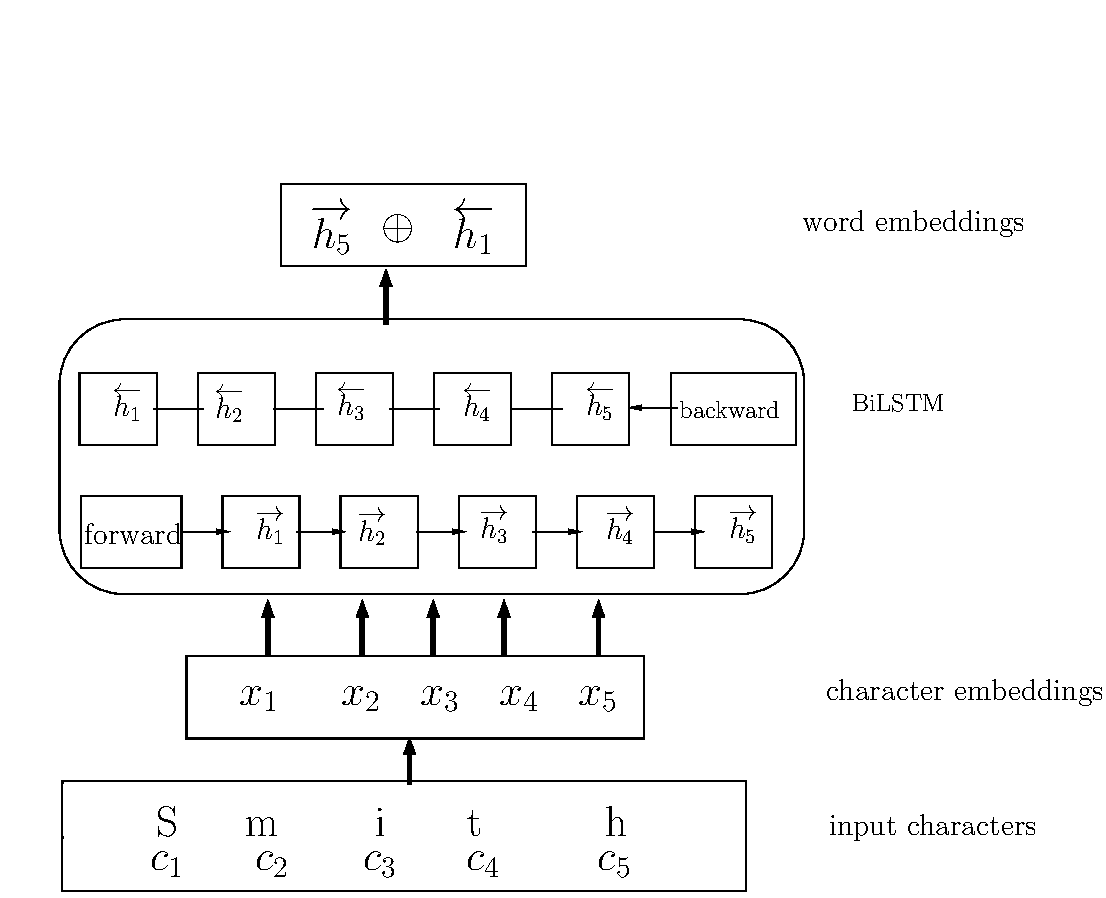
\includegraphics[scale=0.6]{bilstmchar.pdf}
 \caption{The word embedding derived from the character embeddings}
  \label{fig:charlstm}
\end{figure}

\subsection{Conditional Random Fields}

Conditional Random Fields (CRF) models make decisions on sentence levels instead of making independent decisions on each word. We combine the BiLSTM model with a CRF layer to form the BiLSTM-CRF model. In BiLSTM-CRF, given a sequence of output predictions $y=\left( y_{1},y_{2},\ldots y_{n}\right)$, the score of the output sequence is:

\begin{equation}
S\left( y\right)=\sum _{i}^{n}T_{i,i+1}+\sum _{i}^{n}p_{i}\left(y_{i}\right)
\end{equation}

where $T$ is a matrix of transition scores such that $T_{i,j}$ represents the score of a transition from the label $i$ to label $j$, and $p_{i}\left(y_{i}\right)$ is the probability of $y_{i}$ being the label of word $i$.

During training, we score every possible output sequence, and use a softmax layer to generate the probability distribution of output sequences, shown in Equation \ref{eqn:softmax}. Then, we minimize the negative log likelihood over the training sentences. During decoding, we can recover the tag sequences of test data using dynamic programming.

\begin{equation}\label{eqn:softmax}
P\left( y\right) = \textit{softmax}(S\left( y\right))
\end{equation}

BiLSTM-CRF model can effectively make use of the past and future input information and sentence level tag information. Figure shows an example of using BiLSTM-CRF to predict named entity labels.
 
\section{Experiments and Results}

To evaluate BiLSTM models, we run BiLSTM with three configurations on POS and NER: BiLSTM with word features only (BiLSTM); BiLSTM with Character Embeddings (BiLSTM-Char); BiLSTM with Character Embeddings and a CRF layer (BiLSTM-Char-CRF). We report the performance and decoding speed of the models on Penn Treebank data set for POS, and on CoNLL 2003 data set for NER. 

As in the implementation for feedforward models, we implement BiLSTM models using Python and the Tensorflow 1.0 library. The hidden layer size in the BiLSTM of Character Embeddings is set to 50, and the hidden layer size in word sequence BiLSTM is set to 100. The rest of the hyperparameters are the same as the ones in the feedforward network experiments. Since dropout training (\citeauthor{hinton2012improving}, \citeyear{hinton2012improving}) can improve the performance by encouraging the model to depend on both character embeddings and word embeddings, we apply a dropout mask on the input embeddings before the BiLSTM layer. The dropout rate is set to 0.5 in the experiments. Table \ref{table:hyperparameters2} shows the hyperparameters used in BiLSTM models.

\begin{table}[]
\centering
\caption{Hyperparameters used in BiLSTM Models}
\label{table:hyperparameters2}
\begin{tabular}{|c|c|}
\hline
Hyperparameters & Values \\ \hline
character embedding size & 50 \\ \hline
word embedding size & 100 \\ \hline
feedforward layer size & 200 \\ \hline
feedforward layer & 1 \\ \hline
BiLSTM layer size & 100 \\ \hline
BiLSTM layer & 2 \\ \hline 
optimizer & Adam \\ \hline
learning rate & 0.01 \\ \hline
batch size & 32 \\ \hline
\end{tabular}
\end{table}

Figure \ref{fig:lstmbar} illustrates the performance of BiLSTM, BiLSTM-Char, and BiLSTM-Char-CRF. As expected, the fully structured BiLSTM model outperforms the other two. The structure of Character Embeddings increases POS accuracy by 1.17, and increases NER F1 score by 3.34. It reveals that the BiLSTM networks do not heavily depend on features other than words, and Character Embeddings can help improve the performance on NER more than on POS. Compared to BiLSTM-Char, BiLSTM-Char-CRF improves the POS performance by 0.13, and improves the NER performance by 1.79. CRF layer is more helpful for NER for the reason that there are grammar constraints on NER output tag sequence.

\begin{figure}
  \centering
  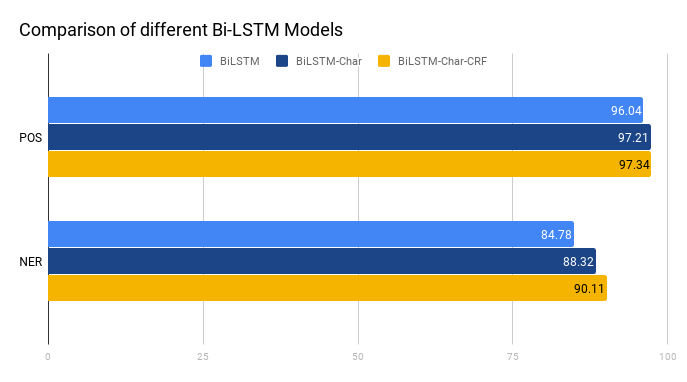
\includegraphics[scale=0.6]{lstmbar.png}
 \caption{Performance comparison between BiLSTM models on POS and NER (accuracy for POS; F1 score for NER}
  \label{fig:lstmbar}
\end{figure}


\begin{table}[]
\centering
\caption{BiLSTM Models Accuracy and F1 Score}
\label{table:lstm-table1}
\begin{tabular}{|c|c|c|}
\hline
Model         & POS (Accuracy)  & NER (F-Score)       \\ \hline
BiLSTM  & 96.01     & 84.78                             \\ \hline
BiLSTM-Char & 97.21 & 88.32             \\ \hline
BiLSTM-Char-CRF & \textbf{97.34}  & \textbf{90.11}             \\ \hline
\end{tabular}
\end{table}

\begin{table}[]
\centering
\caption{BiLSTM Models Decoding Speed}
\label{table:lstm-table2}
\begin{tabular}{|c|c|c|}
\hline
Model       & POS  (sentences, words/sec)  & NER  (sentences, words/sec)      \\ \hline
BiLSTM             & 981(23036)     & 1637(20740)       \\ \hline
BiLSTM-Char        & 596(13992)  & 889(11271)             \\ \hline
BiLSTM-Char-CRF    & 383(9009)  & 795(10100)         \\ \hline
\end{tabular}
\end{table}


Table \ref{table:lstm-table1} and Table \ref{table:lstm-table2} describe the final results of the performance and decoding speed of BiLSTM models on the POS and NER. It is obvious that the more features the model has, the slower it would be. Adding a CRF layer will increase the performance but decrease the decoding speed. 

%Table \ref{table:lstm-table3} compares the fully structured BiLSTM-Char-CRF model with Feedforward-History and Feedforward-CRF. The results reveal that considering the whole sequence in training can improve the performance, but models without recurrent structure or CRF can be faster and achieve comparable accuracy.



\iffalse
\begin{table}[]
\centering
\caption{Decoding Speed Comparison between BiLSTM Models and Feedforward Models on POS and NER}
\label{table:lstm-table3}
\begin{tabular}{|c|c|c|}
\hline
Model       & POS  (sentences, words/sec)  & NER  (sentences, words/sec)      \\ \hline
Feedforward-History            & 829(19474)     & 1390(17609)       \\ \hline
Feedforward-CRF        & 761(17877)  & 1374(17412)             \\ \hline
BiLSTM-Char-CRF    & 383(9009)  & 795(10100)         \\ \hline
\end{tabular}
\end{table}
\fi

